% ==========================================================
\section{Comprehension of Behavioral Programs}
\label{sec:sota_bp_comprehension}
% ==========================================================
 
As Behavioral Programming applications grow in size, understanding why certain events are selected while others are blocked becomes increasingly difficult.
The parallel execution of multiple b-threads, combined with complex event interaction rules, makes it difficult for developers to reason about program behavior or diagnose failures.
To address this comprehensibility challenge, three distinct tools have emerged.
Each targets a different phase of the development lifecycle and offering complementary capabilities for understanding \gls{bp} systems.

% ----------------------------------------------------------
\subsection{Trace Visualization}
\label{subsec:tracevis}
% ----------------------------------------------------------
 
TraceVis~\cite{eitan_visualization_2011} was proposed by Eitan et al.\ 
The tool was already featured alongside the original Behavioral Programming paper~\cite{harel_behavioral_2012}.
It is a web-based, interactive grid display that shows the state of a behavioral program over time (Figure~\ref{fig:tracevis}).
Synchronization points are organized along the rows, while b-threads are organized along the columns, ordered by priority.
Each cell represents the state of a b-thread at a given synchronization point, indicating which b-events are requested, waited-for, or blocked.
Visual cues, such as green stars for selected events and red squares for blocked ones, help developers track the execution flow.
To handle larger applications, TraceVis provides grouping by a b-thread class and filtering mechanisms that allow inactive threads to be hidden.
The tool was designed for the Java implementation of \gls{bp}, BPJ~\cite{harel_programming_2010}, which generates an XML trace file at the end of a run.
Based on the import of this trace file, TraceVis reconstructs the execution history and visualizes it in the browser.
As a result, TraceVis is strictly a post-execution analysis tool with no ability to control or interrupt a live program.

\begin{figure}
	\centering
	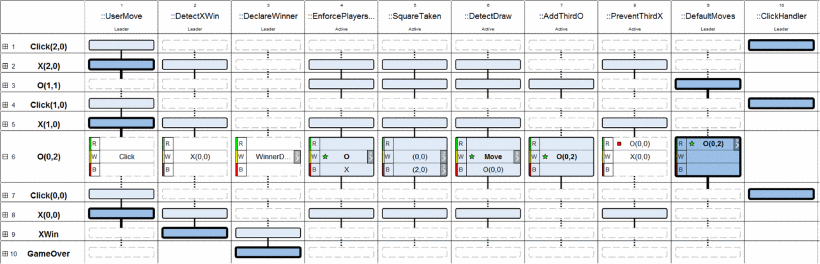
\includegraphics[width=\textwidth]{figures/tracevis.png}
	\caption[Trace Visualization]{Showcase of TraceVis using a Tic-Tac-Toe game. Taken from \cite{eitan_visualization_2011}.}
    \label{fig:tracevis}
\end{figure}
 
% ----------------------------------------------------------
\subsection{Runtime Debugger}
\label{subsec:bp_debugger}
% ----------------------------------------------------------
 
To address the limitations of TraceVis, a runtime debugger for \gls{bp} was subsequently proposed~\cite{felber_debugging_2024}.
It is a web application with a table-like structure for visualising the system state, which is illustrated in Figure~\ref{fig:bp_debugger}.
Rather than consuming a post-run trace file, it hooks directly into the executing program and streams state data to the browser at every synchronization point.
This includes b-threads, b-events, and additional parameters.
The approach provides runtime controls similar to those in symbolic debuggers, including pausing execution and setting conditional breakpoints.
These breakpoints can be chained to halt execution only if a specific sequence of conditions occurs across consecutive synchronization points.
Additionally, the debugger adopts a \textit{models@run.time} approach to incrementally construct an abstracted runtime model in memory~\cite{felber_debugging_2024}.
This model enables time-travel debugging, allowing developers to navigate to arbitrary past system states and trace a bug's origin.
Recorded traces can be exported and re-imported for side-by-side comparison with a live run.

\begin{figure}
	\centering
	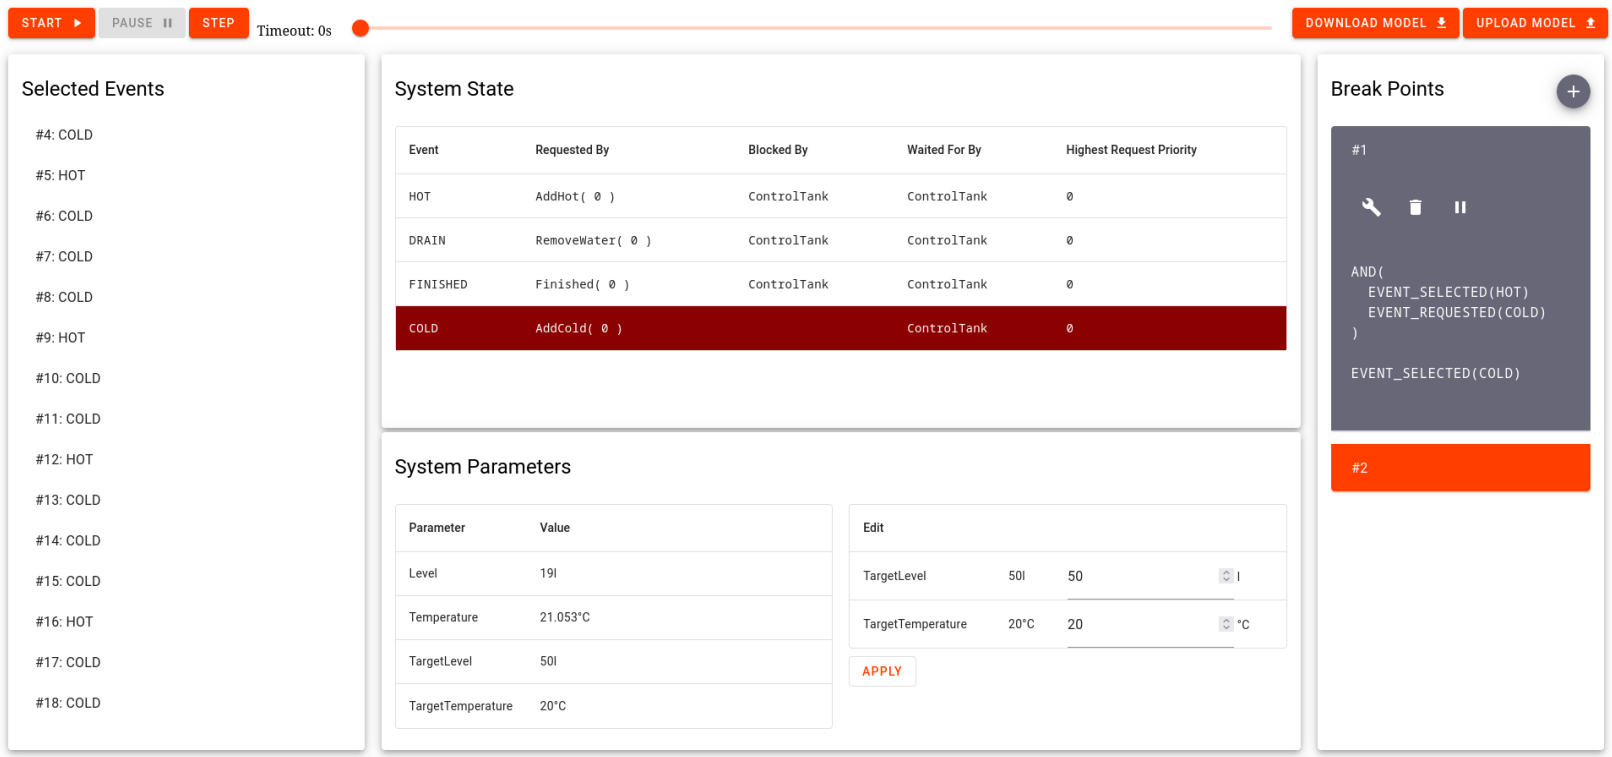
\includegraphics[width=\textwidth]{figures/bp_debugger.png}
	\caption[BP Runtime Debugger]{Main UI of the BP Runtime Debugger. Taken from \cite{felber_debugging_2024}.}
    \label{fig:bp_debugger}
\end{figure}

% ----------------------------------------------------------
\subsection{Feature Modeling for Behavioral Programming}
\label{subsec:fmbp}
% ----------------------------------------------------------
 
FMBP~\cite{felber_comprehensible_2025} addresses comprehensibility at the architectural design phase, before any behavioral code is written.
Rather than analyzing a running or completed program, it provides a formal model of the expected system structure.
FMBP is a Python framework that extends \gls{uvl} to represent \gls{bp} as an architecture description language, modeling b-threads as structural features and their events as feature attributes.
This formal representation enables automated SMT-checking and type verification before implementation, surfacing logical contradictions and constraint violations early.
At runtime, FMBP connects the feature model to the executing program through two components.
The \texttt{ConsistencyChecker} compares the live system state against the expected model structure, while the \texttt{BPConfigurator} reconfigures the behavioral layout in response to dynamic environmental context~\cite{felber_comprehensible_2025}.
Together, these mechanisms provide an overview of expected system interactions across the entire development lifecycle.
 
As part of FMBP, the \gls{uvls} was extended to support \gls{bp}.
B-threads are represented as features, while b-events are modelled as composite feature attributes nested within their respective b-thread features.
Each event attribute carries explicit properties for \texttt{requested}, \texttt{blocked}, \texttt{waited\_for}, and a \texttt{priority} value~\cite{felber_comprehensible_2025}.

Explicit type annotations are required throughout the model to prevent ambiguity and ensure consistency.
A b-thread feature must contain an attribute \texttt{type 'BThread'} to indicate its role, while event attributes must be tagged with \texttt{type 'BEvent'}.
The extended \gls{uvls} enforces strict name-type consistency, ensuring that any parameter passed into a constraint function carries a \texttt{BEvent} type annotation wherever it appears~\cite{felber_comprehensible_2025}.
Semantic errors, such as an event nested inside another event, are surfaced as immediate IDE errors.
 
The extension also defines aggregate constraint functions that translate into SMT-solver expressions for automated verification.
Three basic functions are \texttt{requested()}, \texttt{blocked()}, and \texttt{waited\_for()}.
They query the model to determine whether any b-thread exhibits a specific behavior for a given event.
Two specialized constraints support reasoning about event interactions.
\texttt{conflicting()} enforces mutual exclusion among an arbitrary number of events.
\texttt{selected()} verifies that a specified event is guaranteed to be triggered by analyzing the collective effect of all b-threads' priorities, requests, and blocks~\cite{felber_comprehensible_2025}.

To support context-awareness, FMBP introduces two special top-level features for modeling dynamic behavior and system configuration.
The \texttt{Env} feature holds variables representing runtime environmental state such as sensor readings, system parameters, or external events.
The \texttt{Config} feature provides a top-level container for static configuration parameters that control the behavioral layout independent of runtime context.
Both features can be referenced in constraints to enable context-sensitive behavior selection~\cite{felber_comprehensible_2025}.